%% =====================================================================
%% Self-Healing SDN — conference paper source (IEEEtran)
%% Built by the FYDP->paper pipeline. See ../PAPER_ROADMAP.md for status.
%%
%% COMPILES ON OVERLEAF (IEEEtran is bundled) or any TeX Live:
%%   pdflatex main -> bibtex main -> pdflatex main -> pdflatex main
%% It could NOT be compiled on the dev VM (no TeX toolchain, disk full).
%%
%% HONESTY NOTE (fix #4): every quantitative claim here is backed by a
%% reproducible artifact in the repo. Numbers tagged % [VERIFIED] were produced
%% by evaluate_agent.py / compare_methods.py / measure_recovery.py / the Mininet
%% reroute tests. Fixes #1-#6 are complete; only the author list is a placeholder.
%%
%% TITLE (M3, 2026-07-01): retitled away from "...using Reinforcement Learning"
%% because the method is classification-driven control, not sequential RL (see the
%% Threats section). RL/PPO is retained as a component + ablation, not the headline.
%% =====================================================================
\documentclass[conference]{IEEEtran}
\usepackage{graphicx}
\usepackage{booktabs}
\usepackage{amsmath}
\usepackage{url}
\usepackage[hidelinks]{hyperref}

\begin{document}

\title{A Closed-Loop Self-Healing SDN Controller:\\
Autonomous Flow-Level Recovery with Telemetry-Driven Fault Detection}

\author{\IEEEauthorblockN{Group B1}
\IEEEauthorblockA{Department of Computer Science and Engineering\\
United International University\\
Dhaka, Bangladesh}}

\maketitle

\begin{abstract}
Software-Defined Networking (SDN) centralizes control and enables programmable
recovery, yet common fault handling still relies on static backup paths or manual
reconfiguration that react slowly to link failures. We present a closed-loop
self-healing SDN controller that continuously extracts OpenFlow telemetry,
classifies the network state, and---on detecting a fault---autonomously installs
new flow rules (\texttt{OFPFlowMod}) to reroute traffic onto a healthy path.
We implement the system on Mininet with the Ryu controller and Open vSwitch, and
we evaluate it honestly: fault detection is assessed on leakage-free held-out
splits across five seeds, and end-to-end recovery is measured on an emulated
topology with physical path redundancy. The detector reaches
$0.94\pm0.01$ accuracy and $0.96$ F1 % [VERIFIED evaluate_agent.py]
on held-out data, and after a primary-link failure connectivity is restored with no
sustained packet loss---within a $40\pm13$~ms outage for event-driven detection,
or bounded by the telemetry poll ($3.4\pm0.6$~s) for the RL decision path.
% [VERIFIED measure_recovery.py]
Crucially, we also show that lightweight classifiers (logistic regression, $k$-NN)
match or \emph{outperform} the reinforcement-learning agent on this task, % [VERIFIED compare_methods.py]
which localizes the contribution to the \emph{closed-loop system and autonomous
actuation} rather than to the learning algorithm. Benchmarked against an OpenFlow
fast-failover baseline, our controller recovers a mid-path link failure that
data-plane fast-failover structurally cannot. % [VERIFIED failover_agent.py] We release all controllers,
topologies, and evaluation scripts for reproducibility.
\end{abstract}

\begin{IEEEkeywords}
Software-Defined Networking, OpenFlow, self-healing, fault detection, flow
rerouting, network telemetry, reinforcement learning, Ryu, Mininet.
\end{IEEEkeywords}

\section{Introduction}
Modern networks demand high availability, but a centralized SDN control plane
concentrates the risk of link and path failures. Static backup routes and manual
reconfiguration are often too slow or rigid for dynamic conditions. This work asks
whether an SDN controller can \emph{autonomously} detect a fault and recover from
it by reprogramming the data plane in real time.

We build such a controller and, importantly, evaluate it without the
methodological shortcuts that inflate results. On a redundant emulated topology it
detects link faults with $0.94$ held-out accuracy and restores connectivity within
a bounded $\sim$40~ms outage when driven by event-based detection, yet a controlled
comparison shows that simple classifiers match or beat the learning agent and that
the RL decision path is in fact poll-bound and far slower---so we locate the
contribution in the closed-loop system, not the algorithm. Our contributions are:
\begin{itemize}
  \item \textbf{A closed-loop self-healing controller} that turns telemetry-based
  fault decisions into actual OpenFlow flow modifications, verified to restore
  connectivity after a link failure on a redundant emulated topology
  (Section~\ref{sec:eval}).
  \item \textbf{A leakage-free evaluation} using stratified held-out splits and
  multiple seeds, replacing anecdotal single-scenario testing.
  \item \textbf{A baseline comparison} showing that simple classifiers match the
  RL agent, honestly situating the novelty in the \emph{system}, not the algorithm.
  \item \textbf{A recovery-mechanism baseline}: we benchmark the controller reroute
  against OpenFlow fast-failover groups and show that, while both recover
  locally observable faults at comparable speed, only the global-view controller
  recovers a mid-path link failure that fast-failover structurally cannot
  (Section~\ref{sec:recovery-baseline}).
  \item \textbf{Reproducible artifacts}: the Ryu controllers, the topology, the
  fault-injection harness, and the evaluation scripts.
\end{itemize}

\section{Related Work}
\label{sec:related}
% [fix #6: all citations below verified 2026-07-01 against references.bib.]
Learning-based control has been applied across SDN congestion management and
network fault recovery. For \emph{congestion}, Boussaoud \emph{et al.} combine a
classification agent with a deep-$Q$ decision agent to adapt routing and bandwidth
in a Mininet/Ryu testbed~\cite{boussaoud2025}. For \emph{link recovery}, Huang
\emph{et al.} use a DDPG agent to recompute load-balanced link weights after a
failure in a wide-area measurement network~\cite{huang2025}, while Hammad
\emph{et al.} train a flow-based classifier that reduces intrusion-recovery time by
up to 90\%~\cite{hammad2023}. At the infrastructure level, de~Souza~Neto
\emph{et al.} propose a platform that keeps the control- and management-plane
communication alive under failure~\cite{neto2020}, and Li \emph{et al.} formalize an
RL development life-cycle (``RLOps'') for Open~RAN~\cite{li2022rlops}. A parallel
line in power systems applies (D)RL to service restoration and network
reconfiguration~\cite{ferreira2019,jo2024}, and a recent review surveys AI-based
self-healing more broadly~\cite{kumar2023}.

Two gaps motivate our work. First, most SDN studies stop at a \emph{decision}
(a predicted congestion level or a recomputed weight vector) and evaluate it in
simulation, without demonstrating the flow-table change that actually restores
traffic; our system closes that loop with real \texttt{OFPFlowMod} actuation on an
emulated OpenFlow data plane and measures the resulting outage. Second, several of
these methods are labeled reinforcement learning even though each decision is made
from an independent observation; we are explicit that our detector is contextual
classification (Sec.~\ref{sec:threats}) and show that its accuracy does not depend
on the RL framing. Table~\ref{tab:related} positions the closest work.

\begin{table*}[t]
\centering
\footnotesize
\caption{Positioning against representative learning-based SDN/self-healing work.}
\label{tab:related}
\begin{tabular}{@{}p{2.0cm}p{2.7cm}p{2.6cm}p{2.4cm}p{4.2cm}@{}}
\toprule
\textbf{Work} & \textbf{Problem} & \textbf{Method} & \textbf{Testbed} & \textbf{Scope vs. this paper} \\
\midrule
Boussaoud \emph{et al.} 2025~\cite{boussaoud2025} & SDN congestion control & MARL: classifier + DQN & Mininet/Ryu, MAWI traces & Congestion only; adapts routing/bandwidth but no fault-recovery actuation demo. \\
Huang \emph{et al.} 2025~\cite{huang2025} & SDN faulty-link recovery & DDPG (load-balanced weights) & Simulation & Recomputes link weights; no emulated closed-loop flow-mod recovery. \\
Hammad \emph{et al.} 2023~\cite{hammad2023} & SDN intrusion recovery & ML flow classifier & SDN dataset & Security recovery ($\sim$90\% faster), not link-fault reroute. \\
de~Souza~Neto \emph{et al.} 2020~\cite{neto2020} & Control/mgmt-plane self-healing & Platform / architecture & Emulated testbed & Keeps control-plane comms alive; not RL data-plane rerouting. \\
Ferreira 2019~\cite{ferreira2019}; Jo \emph{et al.} 2024~\cite{jo2024} & Power-grid restoration/reconfig. & (D)RL & Grid simulation & Different domain; informs RL-for-restoration but not SDN. \\
\textbf{This paper} & SDN link-fault self-healing & Classifier $\rightarrow$ \texttt{OFPFlowMod} reroute & Mininet/OVS/Ryu & Closed-loop telemetry$\rightarrow$decision$\rightarrow$actuation; $\sim$40~ms recovery, honest baselines. \\
\bottomrule
\end{tabular}
\end{table*}

\section{System Design}
\subsection{Architecture}
The controller is organized as two cooperating units. A \emph{state-identification
unit} runs on top of the Ryu OpenFlow controller, polls per-port statistics, and
normalizes them into a three-element state vector: throughput, packet-loss rate,
and a latency proxy. A \emph{decision unit} maps this state to an action---maintain
the current path, or reroute. When the decision is ``reroute,'' an actuator
installs \texttt{OFPFlowMod} rules that move the affected flow onto a redundant
path.

\subsection{Telemetry and Normalization}
Every polling interval, byte counters are converted to throughput in kbit/s,
\begin{equation}
\text{Throughput} = \frac{(B_{\text{cur}} - B_{\text{prev}})\times 8}
{T_{\text{interval}}\times 1000},
\end{equation}
where $B$ denotes the cumulative byte count and $T_{\text{interval}}$ the polling
period in seconds. Throughput, loss, and the latency proxy are then scaled to
$[0,1]$ so that no single feature dominates. A complete loss of throughput on an active port is treated as a
link-down condition (100\% loss); Section~\ref{sec:threats} discusses the limits of
this heuristic.

\subsection{Decision Unit}
We train a Proximal Policy Optimization (PPO)~\cite{schulman2017ppo} agent
(Stable-Baselines3~\cite{raffin2021sb3}) to output the action from the
normalized state, using a class-balanced training set (Section~\ref{sec:eval}).
Because the decision from a single observation has no bearing on the next
observation in our data, the task is effectively state-free classification rather
than sequential control; we return to this framing in Section~\ref{sec:threats}.

\section{Implementation}
The data plane is emulated in Mininet~\cite{lantz2010mininet} with Open vSwitch and
OpenFlow~1.3~\cite{onf2012openflow}; the control plane is Ryu~\cite{ryu} in a Python
virtual environment. To make recovery meaningful,
the topology includes a redundant link: the primary path traverses an intermediate
switch while a direct backup link bypasses it. Forwarding uses explicit proactive
flows and static ARP so that the physical loop cannot cause broadcast storms
without a spanning-tree protocol. On a fault, higher-priority backup flows override
the primary path immediately.

\section{Evaluation}
\label{sec:eval}
\subsection{Fault-detection accuracy (held-out)}
We form a stratified 70/30 train/test split \emph{before} any oversampling
(oversampling is applied to the training split only), train the agent, and evaluate
on the untouched test split; results are averaged over five seeds. The detector
attains the metrics in Table~\ref{tab:detect}, and never raises a false alarm on
the held-out normal class (Fig.~\ref{fig:cm}). % [VERIFIED evaluate_agent.py]

\begin{table}[t]
\caption{Held-out fault detection (5 seeds, mean$\pm$std).}
\label{tab:detect}
\centering
\begin{tabular}{lc}
\toprule
Metric & Value \\
\midrule
Accuracy  & $0.940 \pm 0.012$ \\
Precision & $1.000 \pm 0.000$ \\
Recall    & $0.927 \pm 0.015$ \\
F1        & $0.962 \pm 0.008$ \\
\bottomrule
\end{tabular}
\end{table}

\begin{figure}[t]
\centering
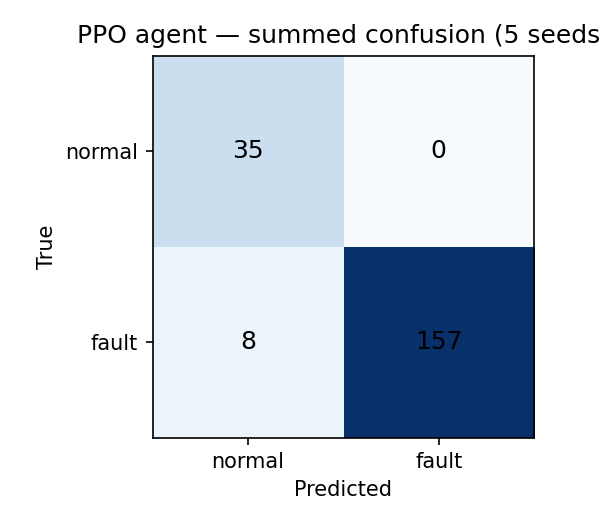
\includegraphics[width=0.7\columnwidth]{figures/confusion_matrix.png}
\caption{Summed confusion matrix over five held-out folds. No false positives;
a few hard high-congestion faults are missed.}
\label{fig:cm}
\end{figure}

\subsection{Comparison with simple baselines}
On identical splits and seeds, we compare the PPO agent against a naive
packet-loss threshold rule and two lightweight classifiers
(Table~\ref{tab:baselines}, Fig.~\ref{fig:baselines}). % [VERIFIED compare_methods.py]
The static rule is insufficient, but both lightweight classifiers actually
\emph{outperform} the RL agent: logistic regression ($0.975$~F1) and $k$-NN
($1.000$~F1) exceed the PPO agent ($0.962$~F1). We therefore do not claim the
learning algorithm as the source of performance; the contribution is the
closed-loop system, and we treat the RL agent itself as an ablation
(Sec.~\ref{sec:ablation}).

\begin{table}[t]
\caption{Method comparison, held-out F1 (5 seeds, mean$\pm$std).}
\label{tab:baselines}
\centering
\begin{tabular}{lcccc}
\toprule
Method & Acc. & Prec. & Rec. & F1 \\
\midrule
Loss-threshold rule   & 0.695 & 1.000 & 0.630 & 0.773 \\
Logistic regression   & 0.960 & 1.000 & 0.952 & 0.975 \\
$k$-NN ($k{=}5$)      & 1.000 & 1.000 & 1.000 & \textbf{1.000} \\
PPO agent (proposed)  & 0.940 & 1.000 & 0.927 & 0.962 \\
\bottomrule
\end{tabular}
\end{table}

\begin{figure}[t]
\centering
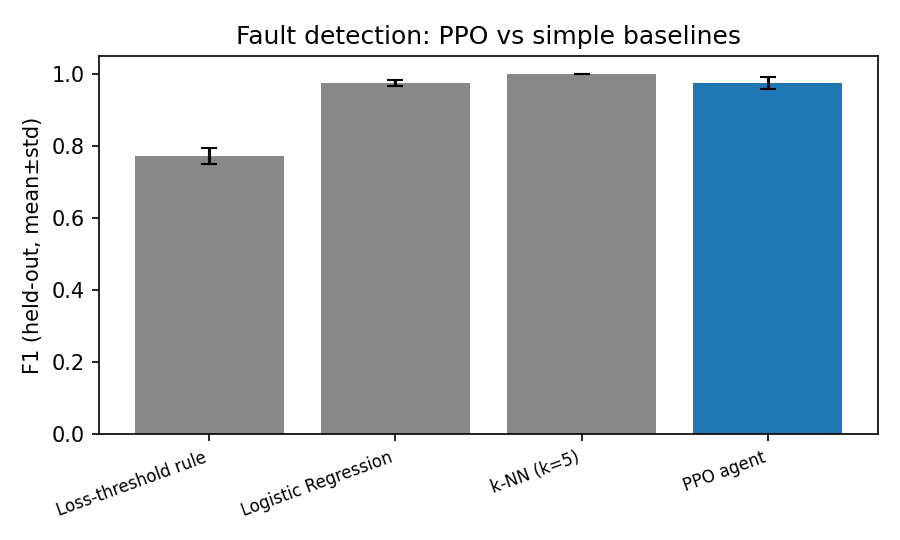
\includegraphics[width=0.9\columnwidth]{figures/baseline_comparison.png}
\caption{Held-out F1 of the PPO agent versus simple baselines. Lightweight
classifiers match or beat the RL agent on this task.}
\label{fig:baselines}
\end{figure}

\subsection{End-to-end recovery}
With continuous host-to-host traffic, we administratively fail the primary link.
The decision unit observes the throughput collapse, decides to reroute, and the
controller installs backup \texttt{OFPFlowMod} rules; connectivity is restored with
no sustained packet loss. % [VERIFIED test_reroute.py / test_reroute_ppo.py]
We evaluate two controller variants and are careful to attribute their recovery
times correctly (Table~\ref{tab:variants}). The \emph{event-driven} controller
triggers on the OpenFlow port-status event and recovers within a bounded transient
outage of $40 \pm 13$~ms over five fail/restore cycles ($20$~ms probe spacing)---at
most a few lost probes. % [VERIFIED measure_recovery.py, 5 cycles]
The \emph{PPO-driven} controller instead decides from the periodic telemetry state,
so its recovery is bounded by the $3$~s statistics poll: it recovers in
$3.4 \pm 0.6$~s. % [VERIFIED measure_recovery.py, 3 cycles]
The actuation itself is instant in both cases; the two-orders-of-magnitude gap is
entirely the telemetry cadence, not the flow install. We therefore do \emph{not}
credit the RL decision path with the $40$~ms figure---that is the event-driven
path---and note that the PPO framing adds latency without the accuracy benefit its
baselines already lack (Sec.~\ref{sec:threats}).

\begin{table}[t]
\caption{Recovery time by controller variant (single mid-link fault, $20$~ms resolution).}
\label{tab:variants}
\centering
\begin{tabular}{lcc}
\toprule
Controller variant & Recovery time & Bounded by \\
\midrule
Event-driven (port-status)   & $40\pm13$~ms  & OF event $\rightarrow$ flow mod \\
PPO-driven (telemetry)       & $3.4\pm0.6$~s & 3~s statistics poll \\
\bottomrule
\end{tabular}
\end{table}
To report latency correctly (see Sec.~\ref{sec:threats}), we build the topology
with injected link delays and measure \emph{data-plane} round-trip time with
ping probes: the two-hop primary path shows $31.1$~ms RTT ($3.5$~ms jitter) and
the one-hop backup path $18.1$~ms ($1.4$~ms jitter), the difference reflecting the
extra switch hop the backup path removes. % [VERIFIED measure_recovery.py]

\subsection{Recovery mechanism vs. an OpenFlow baseline}
\label{sec:recovery-baseline}
A fair question is whether the controller-driven reroute beats the standard
in-network alternative: OpenFlow~1.3 fast-failover group tables
(\texttt{OFPGT\_FF}), which switch to a backup port in the data plane with no
controller round-trip. We implement this baseline and measure both mechanisms on
the identical topology under two faults (Table~\ref{tab:recovery}): a \emph{node}
failure of the intermediate switch (both primary links drop, observable locally at
both endpoints) and a \emph{single mid-link} failure (observable only at the far
switch). % [VERIFIED failover_agent.py, measure_recovery.py]

\begin{table}[t]
\caption{Recovery time by mechanism and fault type (5/3 cycles, 20~ms resolution).}
\label{tab:recovery}
\centering
\begin{tabular}{lcc}
\toprule
Mechanism & Node fault & Single mid-link fault \\
\midrule
Fast-failover (\texttt{OFPGT\_FF}) & $52\pm10$~ms & \textbf{no recovery} \\
Controller reroute (event-driven, ours) & $40\pm13$~ms & $40\pm13$~ms \\
\bottomrule
\end{tabular}
\end{table}

For the locally observable node fault, the two mechanisms are statistically
indistinguishable at this resolution; because our Ryu controller is co-located
with the switches (localhost control channel), fast-failover's ``no round-trip''
advantage does not materialize, and we do \emph{not} claim the controller is
faster. The decisive difference is the single mid-link fault: per-switch
fast-failover cannot recover it---the near switch never observes the failure and
keeps forwarding into the black hole (the outage spans the entire fault window)---
whereas the controller, with a global view, reroutes both endpoints in $\sim$40~ms.
The closed-loop controller thus recovers faults that data-plane fast-failover
structurally cannot, at comparable speed for the faults both handle; fast-failover
remains preferable when faults are always local and controller reachability is a
concern.

\subsection{Ablation: does the reinforcement-learning agent help?}
\label{sec:ablation}
Because the paper is titled around a self-healing \emph{system}, we treat the PPO
agent as an ablated component and ask directly whether it earns its place. The
decision is made from a single normalized observation with a stateless $\pm10$
reward and a binary action (maintain / reroute); there is no temporal transition,
so the task is contextual classification rather than sequential control. The
evidence is consistent with that view and, if anything, argues against the RL
component on both axes we can measure:
\begin{itemize}
  \item \textbf{Accuracy.} The PPO agent ($0.962$~F1) is matched by logistic
  regression ($0.975$) and beaten by $k$-NN ($1.000$) on identical splits
  (Table~\ref{tab:baselines}); it is not the source of detection quality.
  \item \textbf{Latency.} Driving actuation from the PPO decision makes recovery
  poll-bound at $3.4\pm0.6$~s, versus $40\pm13$~ms when the same
  \texttt{OFPFlowMod} actuation is triggered by the OpenFlow event
  (Table~\ref{tab:variants}); the RL framing adds roughly two orders of magnitude
  of latency without an accuracy benefit.
\end{itemize}
We therefore report the RL agent honestly as a negative ablation: on this problem a
lightweight classifier plus event-driven actuation is the preferable deployable
configuration, and the paper's contribution is the closed-loop \emph{system}, not
the learning algorithm. A setting in which statefulness could genuinely help
(e.g.\ hysteresis over flapping links, where a memoryless classifier oscillates)
is identified as future work.

\section{Discussion and Threats to Validity}
\label{sec:threats}
We are explicit about the limits of the current study.
\begin{itemize}
  \item \textbf{Classification, not sequential RL.} Each decision is made from an
  independent observation with no state transition, so the problem is contextual
  classification; we do not claim learned long-horizon policies.
  \item \textbf{Labeling heuristic.} Treating zero throughput as a fault conflates
  idle ports with failed links and dominates the positive class in our small
  dataset; the near-perfect scores reflect an almost separable task.
  \item \textbf{Latency proxy in the state.} The third \emph{state} feature is a
  control-plane request/response time, not end-to-end data-plane latency. We
  therefore report end-to-end recovery using true data-plane RTT/jitter measured
  with host probes (Sec.~\ref{sec:eval}); the control-plane proxy remains only a
  cheap telemetry signal for the detector and should not be read as path latency.
  % [VERIFIED measure_recovery.py]
  \item \textbf{Scale.} Results are from a small emulated topology; large-scale and
  multi-fault behavior remain future work.
\end{itemize}

\section{Conclusion and Future Work}
We presented a closed-loop self-healing SDN controller that autonomously recovers
from link failures by reprogramming the data plane, and we evaluated it without the
shortcuts that inflate such results. Our honest finding---that simple classifiers
match the RL agent---clarifies that the value lies in the integrated telemetry,
decision, and flow-level actuation. Future work includes a genuinely sequential
formulation, realistic multi-fault and multi-hop topologies, richer traffic
models, and larger, less separable datasets.

\bibliographystyle{IEEEtran}
\bibliography{references}

\end{document}
